\chapter{Anisotropy -- H or C or HC}

\section{Theory}
There are situations where the coordinate directions do not align easily with the directions of anisotropy of the medium. In that case, the governing equation of the flow should be written in the more general form.
\begin{figure}[H]
\centering
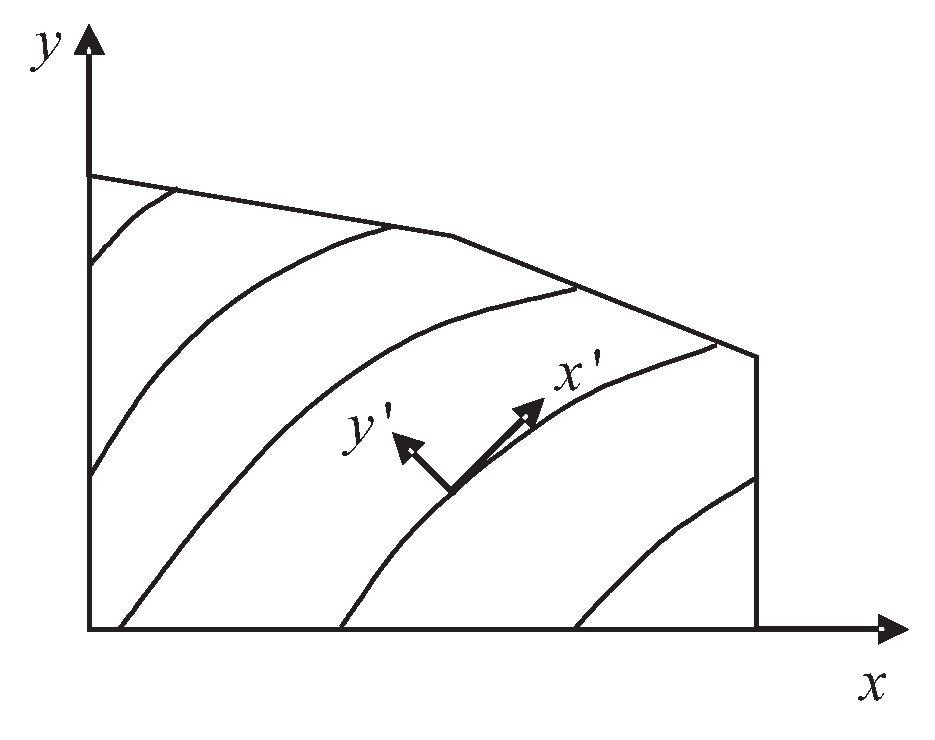
\includegraphics[scale=0.60]{Anisotropy/figures/generalanisotropy.eps}
\caption{General anisotropy system}
\label{GeneralAnisotropy}
\end{figure}
\textbf{Assumption:}

1. The material is isotropic \\
   or \\
2. The coordinate axes coincide with the principal directions of anisotropy. 

For the general case that the coordinate axes do not coincide with the principal directions, the continuity equation is of the form:
\begin{eqnarray}
\label{ani:equ1}
    \frac{\partial }{{\partial x_i }}\left( {K_{ij} \frac{{\partial u}}{{\partial x_j }}} \right) = S\frac{{\partial u}}{{\partial t}}
\end{eqnarray}
where   is the hydraulic conductivity tensor.  Equation \ref{ani:equ1} can be expanded as to:
\begin{eqnarray}
\label{ani:equ2}
\frac{\partial }{{\partial x}}\left( {K_{xx} \frac{{\partial u}}{{\partial x}}} \right) + \frac{\partial }{{\partial x}}\left( {K_{xy} \frac{{\partial u}}{{\partial y}}} \right) + \frac{\partial }{{\partial y}}\left( {K_{yx} \frac{{\partial u}}{{\partial x}}} \right) + \frac{\partial }{{\partial y}}\left( {K_{yy} \frac{{\partial u}}{{\partial x}}} \right) \\ = S\frac{{\partial u}}{{\partial t}\nonumber}
\end{eqnarray}

For a valid solution of the general case, these terms must be included in the numerical procedure, and in finite differences this would be the only available option. In finite elements, we have a second option, which is to rotate the local coordinate axes into the principal directions of hydraulic conductivity. The second option is computationally more efficient, since the terms in the finite element equation are kept to a minimum. This option is preferred where the principal directions are invariant in time, and where the rotation is easily accomplished, as for example in 2D flow problems. Note that the principal directions can be different for each element. This feature is particularly useful for cross-sectional systems with complex stratification. \\
The rotation is performed for each element individually. The nodal coordinates on the element are rotated (Figure \ref{RotationOfAxes}) according to:
\begin{eqnarray}
    \left\{ {\begin{array}{*{20}c}
   {x'}  \\
   {y'}  \\
\end{array}} \right\} = \left[ {\begin{array}{*{20}c}
   {\cos \beta } & {\sin \beta }  \\
   { - \sin \beta } & {\cos \beta }  \\
\end{array}} \right]\left\{ {\begin{array}{*{20}c}
   x  \\
   y  \\
\end{array}} \right\}
\end{eqnarray}

where  $x'$ , $y'$ are the coordinates of the point  $x$ , $y$ in the principal direction coordinate system, and  $\beta $ is the angle between the Cartesian axes and the principal axes. The angle can be different for each element.

\begin{figure}[H]
\centering
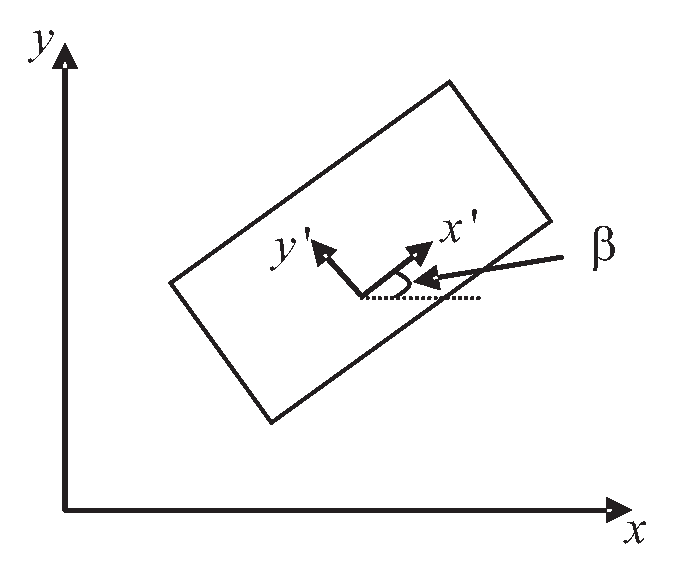
\includegraphics[scale=0.60]{Anisotropy/figures/rotation.eps}
\caption{Rotation of axes}
\label{RotationOfAxes}
\end{figure}

The same theory for anisotropy can be applied to any tensor material properties such as molecular diffusion coefficients.

\section{Anisotropic permeability for pressure or hydraulic head}

Knowing the theoretical background in 9.1, we formulate a simple flow problem to show the difference of three results obtained from isotropic, orthotropic, and anisotropic flow conditions.

\textbf{Problem definition:}

A unit square of the porous medium is created and discretized with triangle elements as in Figure \ref{BCandGrid}. To generate flow in the model domain, two constant pressure boundary conditions are applied to the top left corner and the bottom right corner. The pressure difference between these two points is set to be unity.
\begin{figure}[H]
\centering
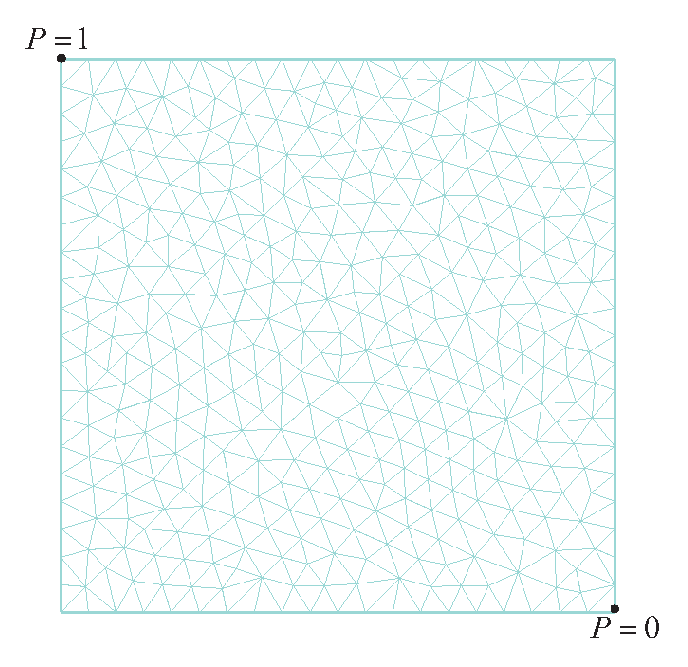
\includegraphics[scale=0.60]{Anisotropy/figures/grid.eps}
\caption{Boundary conditions and grid}
\label{BCandGrid}
\end{figure}

As for material properties for flow system, permeability is set to have isotropic, orthotropic, and anisotropic over the whole model domain and provided in Table \ref{tab:materials_permeability}.

\begin{table}[!htb]
\label{tab:materials_permeability}
\centering
\begin{tabular}{ll}
\hline\hline
{\smallskip}
Material Types & Permeability( $m^2$ ) \\
\hline
Isotropic & $k_{xx}  = k_{yy}  = 10^{ - 14} $ and $k_{xy}  = k_{yx}  = 0$ \\
Orthotropic & $k_{xx}  = 10^{ - 14} ,\,\,k_{yy}  = 10^{ - 15} \,,\,\,and\,k_{xy}  = k_{yx}  = 0$ \\
Anisotropic    & $k_{xx}  = 5.5 \times 10^{ - 15} ,\,\,k_{xy}  = 4.5 \times 10^{ - 15} ,\,\,k_{yx}  = 4.5 \times 10^{ - 15} ,\,\,$ \\
&$k_{yy}  = 5.5 \times 10^{ - 15}$\\
\hline\hline
\end{tabular}
\caption{Various flow types set by material properties}
\end{table}

Anisotropic ratio is set to be 10 to 1 for the $x$ and $y$ axes respectively for the orthotropic case while the anisotropic case uses the same ratio for the $x'$ and $y'$ axes rotated $45^ \circ  $ counter-clock-wise from the $x$ and $y$ axes.\\
The resulting pressure distributions for the three different flow system are provided in Figure \ref{AnisotropicPermeability}.
\begin{figure}[H]
\centering
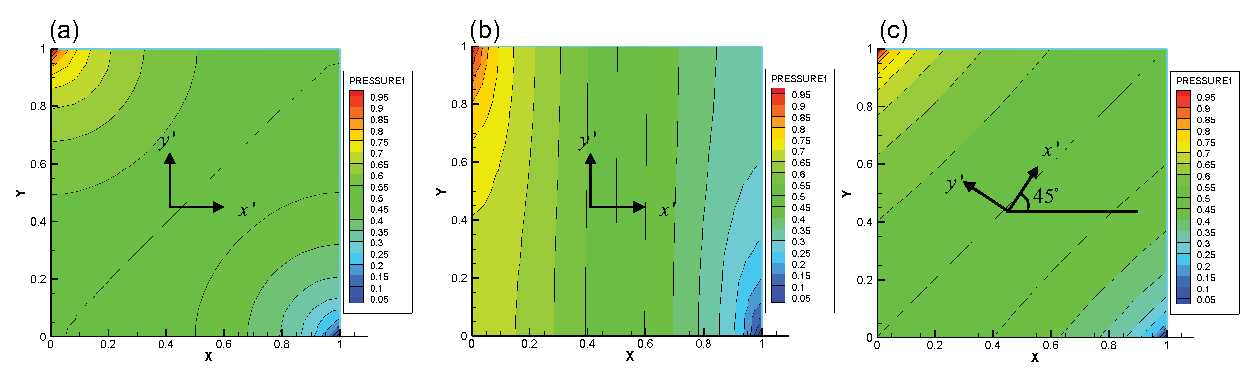
\includegraphics[scale=0.60]{Anisotropy/figures/anisotropicpermeability.eps}
\caption{Pressure distributions for (a) isotropic, (b) orthotropic, and (c) anisotropic permeability}
\label{AnisotropicPermeability}
\end{figure}

Note that there is no technical difference between the orthotropic and anisotropic cases when full values of permeability tensor are given and set into GeoSys/Rock \\Flow. However, users have two options for orthotropic cases in setting up .mmp files using different keywords such as ORTHOTROPIC and ANISOTROPIC.  In the case that diffusion coefficients are treated as tensor via tortuosity, ORTHOTROPIC keyword is no longer valid. Therefore, ANISOTROPIC keyword should be used for Case (b) in anisotropic diffusion via tortuosity.

\subsubsection*{Benchmark deposit}
\begin{tabular}{|l|l|l|}
  \hline
  Benchmark & Problem type & Path in benchmark deposit \\
  \hline
 \emph{soil\_layer}& Anisotropy & benchmarks\verb \Anisotropy\permeability \\
  \hline
\end{tabular}

\section{Anisotropic tortuosity for molecular diffusion coefficients}
As mentioned previously, the theory is exactly same with permeability. One thing to note before introducing another benchmark problem for anisotropic diffusion is that there is clear distinction between hydrodynamic dispersion and molecular diffusion. Since the hydrodynamic dispersion for mass transport in porous media is mainly a function of velocity and dispersivity, the hydrodynamic dispersion may be influenced more significantly by anisotropic hydraulic conductivity as well as pressure distributions than molecular diffusion. However, the hydrodynamic dispersion has also the molecular diffusion term. In this section, this molecular diffusion is treated as tensor via tortuosity that is a material property for instance clay.

The dispersion tensor can be written as (Bear, 1979)
\begin{eqnarray}
\mathord{\buildrel{\lower3pt\hbox{$\scriptscriptstyle\frown$}}
\over D}  = \tau D_m \hat \delta  + \alpha _T \left| v \right|\hat \delta  + \left( {\alpha _L  - \alpha _T } \right)\frac{{\vec v_i \vec v_j }}{{\left| v \right|}}
\end{eqnarray}
where $ \tau $ is the tortuosity tensor $(-) $, $ D_m $  is the coefficient of molecular diffusion $(L^2 T) $, $ \mathord{\buildrel{\lower3pt\hbox{$\scriptscriptstyle\frown$}} \over \delta } $ is the Kronecker-delta (unit tensor) $(-) $,  $ \alpha _T $ is the transverse dispersivity  $(L) $,  $ v $ is the characteristic value of macroscopic velocity $ (LT^{ - 1} ) $, $ \alpha _L $  is the longitudinal dispersivity $(L) $, and, $ \vec v_i $  and $ \vec v_j $ are the velocities in $ i $ and $ j $ directions respectively $ (LT^{ - 1} ) $.


\textbf{Problem definition:}

On the unit square of the porous medium created for the previous flow system, as well as one constant concentration boundary condition is applied, a constant line source is introduced to study the difference of component diffusive transport in various types of media. The transport boundary and source condition are depicted in Figure \ref{gridtransport}.
\begin{figure}[H]
\centering
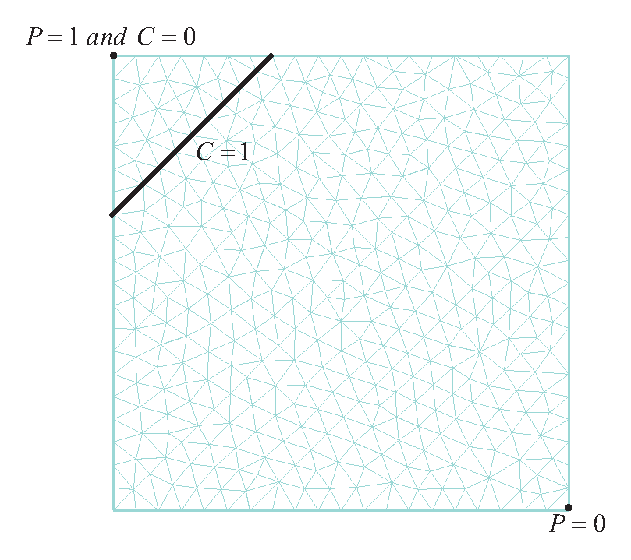
\includegraphics[scale=0.60]{Anisotropy/figures/gridtransport.eps}
\caption{Boundary conditions and a line source for transport model}
\label{gridtransport}
\end{figure}

As for material properties for molecular diffusive transport, tortuosity is set to have isotropic and anisotropic over the whole model domain and provided in Table \ref{tab:materials_tortuosity}.

\begin{table}[!htb]
\label{tab:materials_tortuosity}
\centering
\begin{tabular}{ll}
\hline\hline
{\smallskip}
Material Types & Tortuosity \\
\hline
Isotropic & $\tau _{xx}  = \tau _{yy}  = 1\,\,and\,\,\tau _{xy}  = \tau _{yx}  = 0$ \\
Anisotropic    & $\tau _{xx}  = 0.55,\,\,\tau _{xy}  = 0.45,\,\,\tau _{yx}  = 0.45,\,\,$ \\
&$\tau _{yy}  = 0.55$ : $45^ \circ  $ CCW \\
& $\tau _{xx}  = 0.55,\,\,\tau _{xy}  =  - 0.45,\,\,\tau _{yx}  =  - 0.45,\,\,$ \\
&$\tau _{yy}  = 0.55$ : $135^ \circ  $ CCW\\
\hline\hline
\end{tabular}
\caption{Isotropic and anisotropic tortuosity set for the componential molecular diffusive transport}
\end{table}

An anisotropic ratio is set to be 10 to 1 for the $x'$ and $y'$ axes rotated $45^ \circ  $ counter-clock-wise from the general directions. The equivalent tortuosity expression in the principal directions of anisotropic tortuosity in general coordinate system can be given as

\begin{eqnarray}
\tau '\left( {x',y'} \right) = \left[ {\begin{array}{*{20}c}
   1 & 0  \\
   0 & {1.0}  \\
\end{array}} \right] &  \to  & \tau \left( {x,y} \right) = \left[ {\begin{array}{*{20}c}
   {0.55} & {0.45}  \\
   {0.45} & {0.55}  \\
\end{array}} \right]
\end{eqnarray}

The resulting concentration contours for the three different material systems are provided in Figure \ref{anisotropictransport}.

\begin{figure}[H]
\centering
\includegraphics[scale=0.6]{Anisotropy/figures/anisotropictransport.eps}
\caption{Concentration contours at $t = 1.0 \times 10^8 $ seconds for (a) the isotropic, (b) anisotropic media (45 degrees rotated CCW), and (c) (135 degrees rotated CCW)}
\label{anisotropictransport}
\end{figure}

Finally, the medium is configured to have one bedding subject to anisotropic diffusive transport and all the rest model domain isotropic as depicted in Figure \ref{layeredanisotropictransport}. The resulting concentration contours for this bedding problem is also provided in Figure \ref{layeredanisotropictransport}.

\begin{figure}[H]
\centering
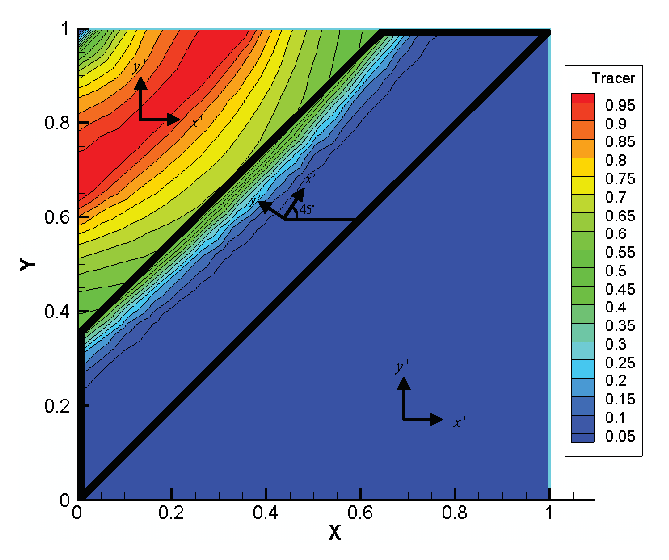
\includegraphics[scale=0.60]{Anisotropy/figures/layeredanisotropictransport.eps}
\caption{Concentration contours at $t = 1.0 \times 10^8 $ seconds for the porous medium with an anisotropic bedding}
\label{layeredanisotropictransport}
\end{figure}

\subsubsection*{Benchmark deposit}
\begin{tabular}{|l|l|l|}
  \hline
  Benchmark & Problem type & Path in benchmark deposit \\
  \hline
 \emph{soil\_layer}& Anisotropy & benchmarks\verb \Anisotropy\moleculardiffusion \\
  \hline
\end{tabular}

\section{Converting an angle of orientation to tensor}
Currently, a universal function for converting an arbitrary angle to tensor is not written yet. In obtaining full tensor values from orthotropic tensor in the global coordinates, the direction of rotation and the magnitude of the angle should be handled carefully. The direction of rotation is counter-clock-wise and the reference tensor should be an identity matrix. Then, the converting function can be written such that

\begin{eqnarray}
\label{ani:TransformMatrix}
K = T^t K'T
\end{eqnarray}

Note that one anisotropic material rotated 180 degrees CCW becomes exactly same anisotropic material. This is obvious from Equation \ref{ani:TransformMatrix}, because 180 degrees produce exactly same matrix $K$.
To clarify the conversion, one example is prepared and explained in Figure \ref{ani:tensordiagram}. Suppose that an anisotropic medium has the ratio of 10 (i.e., $10x' = y'$ , to satisfy this ratio, we can make countless tensors. Thus, we set $\left[ {\begin{array}{*{20}c}   1 & 0  \\  0 & {0.1}  \\ \end{array}} \right]$ for conversion). Note that we talk about anisotropy in principle coordinates thus the coordinate system is single quotation marked. Now we can arbitrally select rotation angles. Figure \ref{ani:tensordiagram} shows some geometrically meaningful angles together with transformed matrix of Equation \ref{ani:TransformMatrix}.

\begin{figure}[H]
\centering
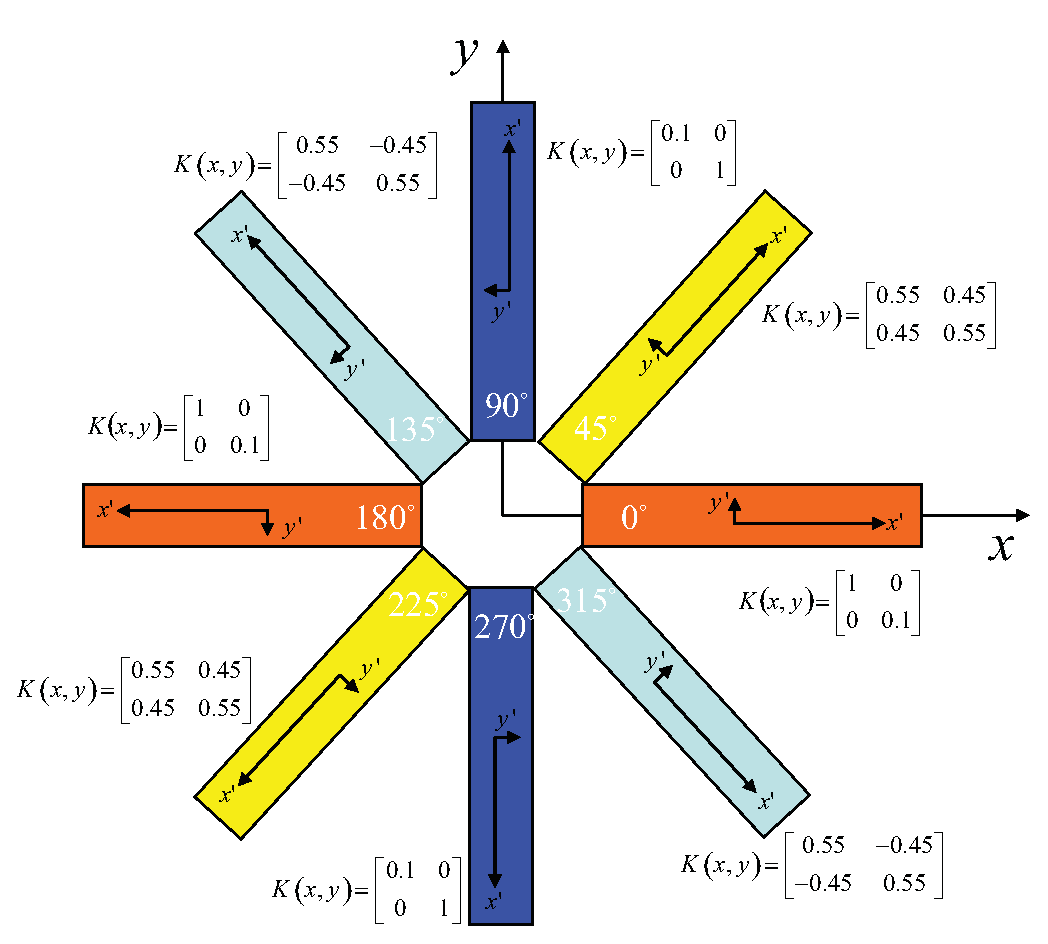
\includegraphics[scale=0.60]{Anisotropy/figures/tensordiagram.eps}
\caption{Transformed tensors referenced from
%{\begin{array}{*{20}c}   1 & 0  \\  0 & {0.1}  \\ \end{array}}
[1 , 0][0 , 0.1]
in the principle coordinates}
\label{ani:tensordiagram}
\end{figure}

In extension to the second rank tensors in other words three dimensions, this direction of the rotation, the magnitude of the two angles, and the rotating axes should carefully be defined when the angles are used to compute the corresponding tensors internally. The transform matrix for three dimensions rotated along the $y$ axis with  $\alpha$ degrees CCW and the $x$ axis with $\beta$ degrees CCW can be written as

\begin{eqnarray}
\label{ani:TransformMatrix3D}
T = \left[ {\begin{array}{*{20}c}
   {\cos \alpha } & {\sin \alpha \sin \beta } & { - \cos \alpha \sin \beta }  \\
   0 & {\cos \beta } & {\sin \beta }  \\
   {\sin \alpha } & { - \cos \alpha \sin \beta } & {\cos \alpha \cos \beta }  \\
\end{array}} \right]
\end{eqnarray}

Since the determinant of $T$ is unity, we can use Equation \ref{ani:TransformMatrix} to compute full tensor values.
This universal converting function will be provided in the future. Until then, full values of tensor should be used in GeoSys/RockFlow for simulating anisotropic problems.
